\chapter{Programas escritos en Lamport}
En este capítulo se definen algunos ejemplos de programas escritos en el lenguaje Lamport y su resultado de ejecución, con el objetivo de mostrar el correcto funcionamiento del intérprete:

\section{Ejemplos secuenciales}
Los siguientes ejemplos mostrados aquí no necesitan de concurrencia para funcionar, pues siguen la estructura y sintaxis básica de cualquier otro programa desarrollado en cualquier lenguaje de alto nivel convencional:

\subsection{Ejemplo 1: Operaciones aritméticas}
\begin{lstlisting}[style=lamportStyle]
{Programa: arithmetic_operations.lmp}
{Autor: Daniel Perez Ruiz}

program Operaciones
	var num1 : integer := (-4 + 6) * 10 - 2;
	var num2 : real := 3.0;

process Main;
	var num3 : integer := 5;
	var num4 : real := (3.5 * 4.2) + (6.7 - 2.3) / 1.1;
begin
	print("num1 tiene de valor: ",num1);
	print("num3 tiene de valor: ",num3);
	print("");
	
	print("num1 + num3 = ",num1+num3);
	print("num1 - num3 = ",num1-num3);
	print("num1 * num3 = ",num1*num3);
	print("num1 / num3 = ",num1/num3);
	print("num1 % num3 = ",num1%num3);
	print("-num1 = ",-num1);
	
	print("");
	
	print("num2 tiene de valor: ",num2);
	print("num4 tiene de valor: ",num4);	
	print("");
	
	print("num2 + num4 = ",num2+num4);
	print("num2 - num4 = ",num2-num4);
	print("num2 * num4 = ",num2*num4);
	print("num2 / num4 = ",num2/num4);
	print("-num4 = ",-num4);
	
end
\end{lstlisting}
\begin{figure}[h]
\caption{Programa Lamport: Operaciones Aritméticas (arithmetic\_operations.lmp)}
\label{fig:lamportArithmeticOperations}
\end{figure}

\newpage
\begin{figure}[h]
    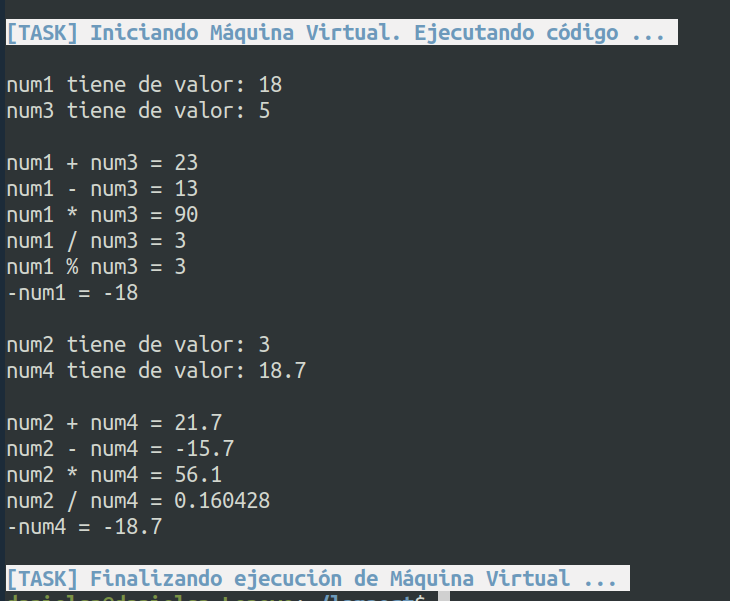
\includegraphics[width=\linewidth]{images/ejemplos/arithmeticOperations.png}
    \caption{Ejecución de arithmetic\_operations.lmp.}
    \label{fig:lamportArithmeticOperations_exec}
\end{figure}

\newpage
\subsection{Ejemplo 2: Operaciones lógicas}
\begin{lstlisting}[style=lamportStyle]
{Programa: logical_operations.lmp}
{Autor: Daniel Perez Ruiz}

program Operaciones
	var a : boolean := true;
	var b : boolean := false;

process Main;
	var c : boolean := true;
begin
	print("a es: ",a);
	print("b es: ",b);
	print("c es: ",c);
	print("");
	
	print("a y b es: ",a and b);
	print("a y c es: ",a and c);
	print("a y b y c es: ",a and b and c);
	print("");
	
	print("a o b es: ",a or b);
	print("a o c es: ",a or c);
	print("a o b o c es: ",a or b or c);
	print("");
	
	print("(a o b) y c es: ", (a or b) and c);
	print("(a o c) y b es: ", (a or c) and b);
	print("");
	
	print("no a es: ",not a);
	print("no b es: ",not b);
	
end
\end{lstlisting}
\begin{figure}[h]
\caption{Programa Lamport: Operaciones Lógicas (logical\_operations.lmp)}
\label{fig:lamportLogicalOperations}
\end{figure}

\newpage
\begin{figure}[h]
    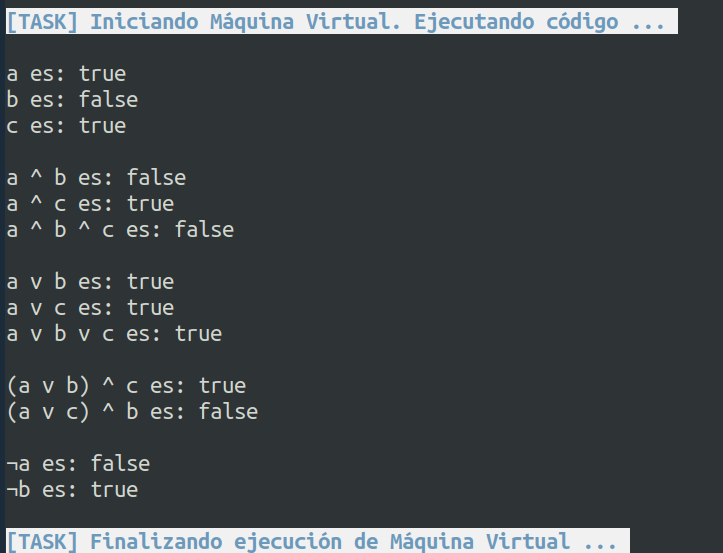
\includegraphics[width=\linewidth]{images/ejemplos/logical_operations.png}
    \caption{Ejecución de logical\_operations.lmp.}
    \label{fig:lamportLogicalOperations_exec}
\end{figure}

\newpage
\subsection{Ejemplo 3: If/Else}
\begin{lstlisting}[style=lamportStyle]
{Programa: ifelse.lmp}
{Autor: Daniel Perez Ruiz}

program CompruebaEdad
	var nombre1 : string := "Jorge";
	var edad1 : integer := 17;
	
	var nombre2 : string := "Pablo";
	var edad2 : integer := 22;
	
process main;
	var minimaEdad : integer := 18;
begin
	print(nombre1, ", tu edad es: ",edad1,". Comprobando si puedes entrar...");
	
	if edad1 < minimaEdad then
		begin
			print("NO puedes entrar. Debes tener ",minimaEdad," para poder entrar.");
		end
	else
		begin
			print("Adelante!!. Puedes entrar");
		end
		
	print("");
		
	print(nombre2, ", tu edad es: ",edad2,". Comprobando si puedes entrar...");
	
	if edad2 < minimaEdad then
		begin
			print("NO puedes entrar. Debes tener ",minimaEdad," para poder entrar.");
		end
	else
		begin
			print("Adelante!!. Puedes entrar");
		end
end
\end{lstlisting}
\begin{figure}[h]
\caption{Programa Lamport: Flujos de control if/else (if\_else.lmp)}
\label{fig:lamportIfElse}
\end{figure}

\newpage
\begin{figure}[h]
    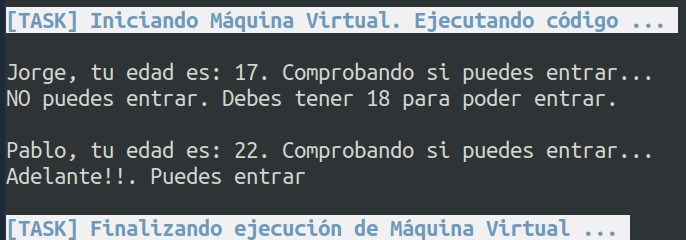
\includegraphics[width=\linewidth]{images/ejemplos/if_else.png}
    \caption{Ejecución de logical\_operations.lmp.}
    \label{fig:lamportIfElse_exec}
\end{figure}

\newpage
\subsection{Ejemplo 4: For}
\begin{lstlisting}[style=lamportStyle]
{Programa: for.lmp}
{Autor: Daniel Perez Ruiz}

program Bucles
	var contador : integer := 5;

process main;
	var startFor : integer := 1;
	var endFor : integer := 5;
begin
	print("La variable contador empieza en: ",contador);
	print("");
	print("Bucle for empieza en: ",startFor);
	print("Bucle for acaba en: ",endFor);
	
	print("");
	
	for i := startFor to endFor do
	begin
		contador := contador+1;
		print("--- contador vale ahora: ",contador);
		print("--- i vale: ", i);
	end
	
	print("");
	print("Ejecutando bucles anidados ...");
	print("");
	
	for j := 1 to 3 do
	begin
		print("------ j vale: ",j);
		for k := j to 4 do
		begin
			print("--- k vale: ",k);
		end
		print("");
	end
	
end
\end{lstlisting}
\begin{figure}[h]
\caption{Programa Lamport: Bucles for (for.lmp)}
\label{fig:lamportFor}
\end{figure}

\newpage
\begin{figure}[!h]
    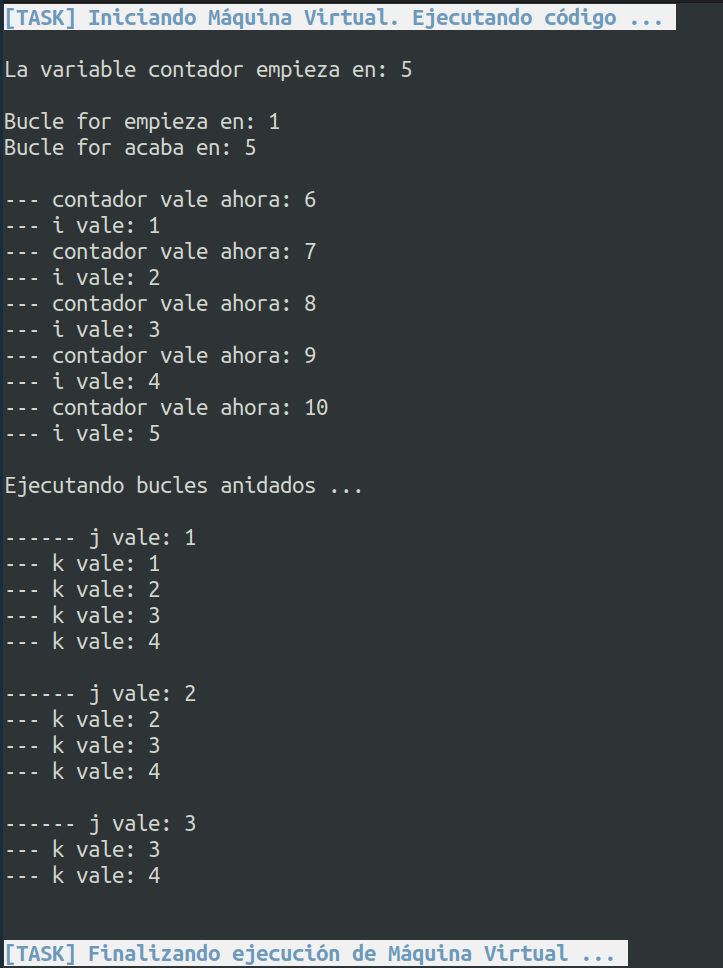
\includegraphics[scale=0.5]{images/ejemplos/for.png}
    \caption{Ejecución de for.lmp.}
    \label{fig:lamportFor_exec}
\end{figure}

\newpage
\subsection{Ejemplo 5: While}
\begin{lstlisting}[style=lamportStyle]
{Programa: while.lmp}
{Autor: Daniel Perez Ruiz}

program Bucles
	var contador : integer := 5;

process main;
	var valorMaximo : integer := 10;
begin
	print("La variable contador empieza en: ",contador);
	print("Su valor maximo debe ser: ",valorMaximo);
	print("");
	
	while contador < valorMaximo do
	begin
		contador := contador + 1;
		print(" --- Contador vale ahora: ", contador);
	end
	
	print(""); print("Fin de bucle");
end
\end{lstlisting}
\begin{figure}[h]
\caption{Programa Lamport: Bucles while (while.lmp)}
\label{fig:lamportWhile}
\end{figure}

\newpage
\begin{figure}[h]
    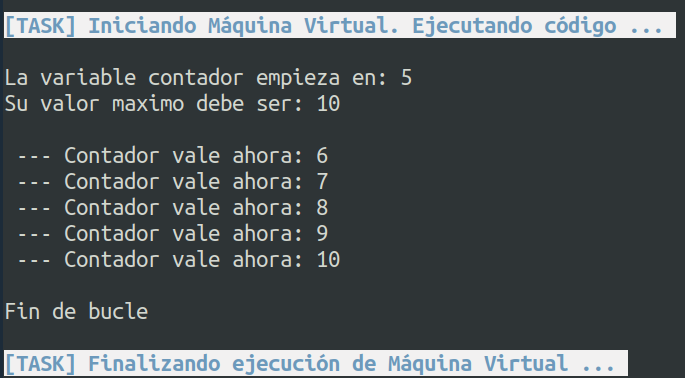
\includegraphics[width=\linewidth]{images/ejemplos/while.png}
    \caption{Ejecución de while.lmp.}
    \label{fig:lamportWhile_exec}
\end{figure}

\newpage
\subsection{Ejemplo 6: Uso de arrays}
\begin{lstlisting}[style=lamportStyle]
{Programa: for.lmp}
{Autor: Daniel Perez Ruiz}

program Arrays
	var numeros : array [5] integer;
process main;
	var letras : array [3] char;
begin
	print("Asignando numeros pares a array de numeros...");
	for i := 0 to 4 do
	begin
		print("Asignando a numeros[",i,"] el valor ",2*i);
		numeros[i] := 2*i;
	end
	
	print("");
	print("Imprimiendo array de numeros...");
	for j := 0 to 4 do
	begin
		print("numeros[",j,"] = ",numeros[j]);
	end
	
	letras[1] := 'd';
	print("");
	print("letras[1] es : ",letras[1]);
end
\end{lstlisting}
\begin{figure}[h]
\caption{Programa Lamport: Uso de arrays (array.lmp)}
\label{fig:lamportArray}
\end{figure}

\newpage
\begin{figure}[h]
    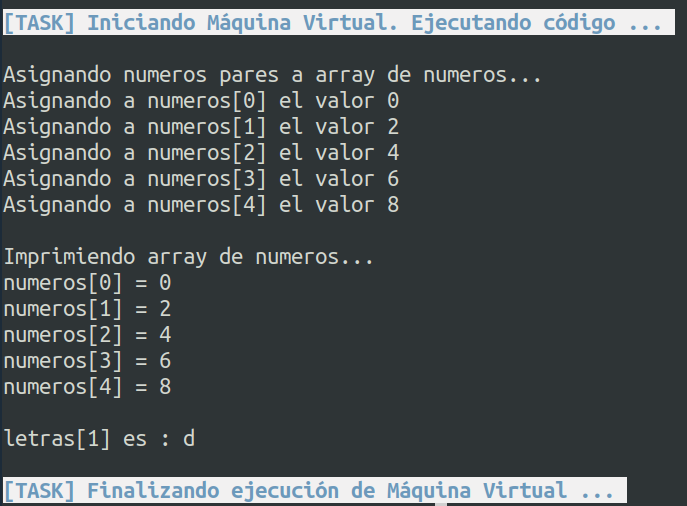
\includegraphics[width=\linewidth]{images/ejemplos/array.png}
    \caption{Ejecución de array.lmp.}
    \label{fig:lamportArray_exec}
\end{figure}

\newpage
\section{Ejemplos que lanzan errores}
Los siguientes ejemplos mostrados son incorrectos, ya sean sintáctica o semánticamente, por lo que el intérprete lanzará los pertinentes mensajes de error.

\subsection{Ejemplo 1: Errores sintácticos en declaraciones}
\begin{lstlisting}[style=lamportStyle]
{Fichero: err_syntax_declarations.lmp}
{Autor: Daniel Perez Ruiz}
{Descripcion: Errores sintacticos de declaraciones}

program SyntaxErrors
	{CORRECTO}
	var v1 : integer;
	var v2 : string := "Hola";
	{ERROR}
	v3 : real;
	var 4v : boolean;
	var v5 char;
	var v6: string

process Main;
	{ERROR}
	var v7 : inventado;
	var v9 : array [5] invent;
	var v10 : integer := ;
	var v11 : integer 2+3;
	var v12 : integer := 1
begin
	print("Syntax errors!");
end
\end{lstlisting}
\begin{figure}[h]
\caption{Programa Lamport: Errores sintácticos (err\_syntax\_decl.lmp)}
\label{fig:lamportErrSintaxDecl}
\end{figure}

\newpage
\begin{figure}[h]
    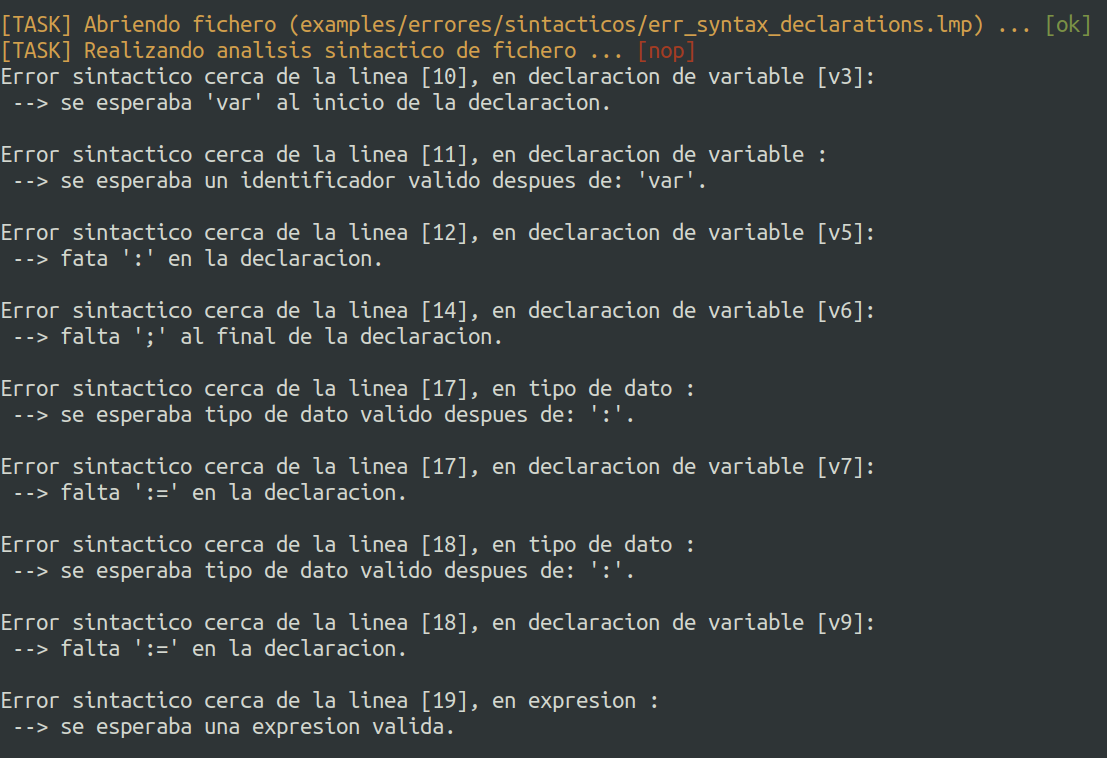
\includegraphics[width=\linewidth]{images/ejemplos/err_syntax/declarations.png}
    \caption{Ejecución de err\_syntax\_decl.lmp.}
    \label{fig:lamportErrSintaxDecl_exec}
\end{figure}

\newpage
\subsection{Ejemplo 2: Errores sintácticos en procedimientos}
\begin{lstlisting}[style=lamportStyle]
{Fichero: err_syntax_procedure.lmp}
{Autor: Daniel Perez Ruiz}
{Descripcion: Errores sintacticos de procedimientos}

program SyntaxErrors

{CORRECTO}
procedure imprimeEdad(a : string, b : integer);
begin
	print("Hola ",a,", tu edad es: ",b);
end

{CORRECTO}
procedure saluda();
begin
	print("hola");
end

{ERROR}
procedure proc1()
begin
	print("proc1");
end

{ERROR}
procedure 2proc();
	var v2 : invent;
begin
	print("fallo");
end

{ERROR}
procedure proc3(a : integer)
begin
	print("valor: ",a);
end

{ERROR}
procedure proc4(2 : integer);
begin
	print("fallo");
end

{ERROR}
procedure proc5(a char);
begin
	print("fallo");
end

{ERROR}
procedure proc6(a : invent);
begin
	print("fallo");
end

{ERROR}
procedure proc7(a : integer, b : invent);
begin
	print("fallo");
end

{ERROR}
procedure proc8(a : char,);
begin
	print("fallo");
end

process Main;
	{ERROR}
	var v1 : invent;
begin
	print("Syntax Errors!");
end
\end{lstlisting}
\begin{figure}[h]
\caption{Programa Lamport: Errores sintácticos (err\_syntax\_procedure.lmp)}
\label{fig:lamportErrSintaxProcedure}
\end{figure}

\newpage
\begin{figure}[h]
    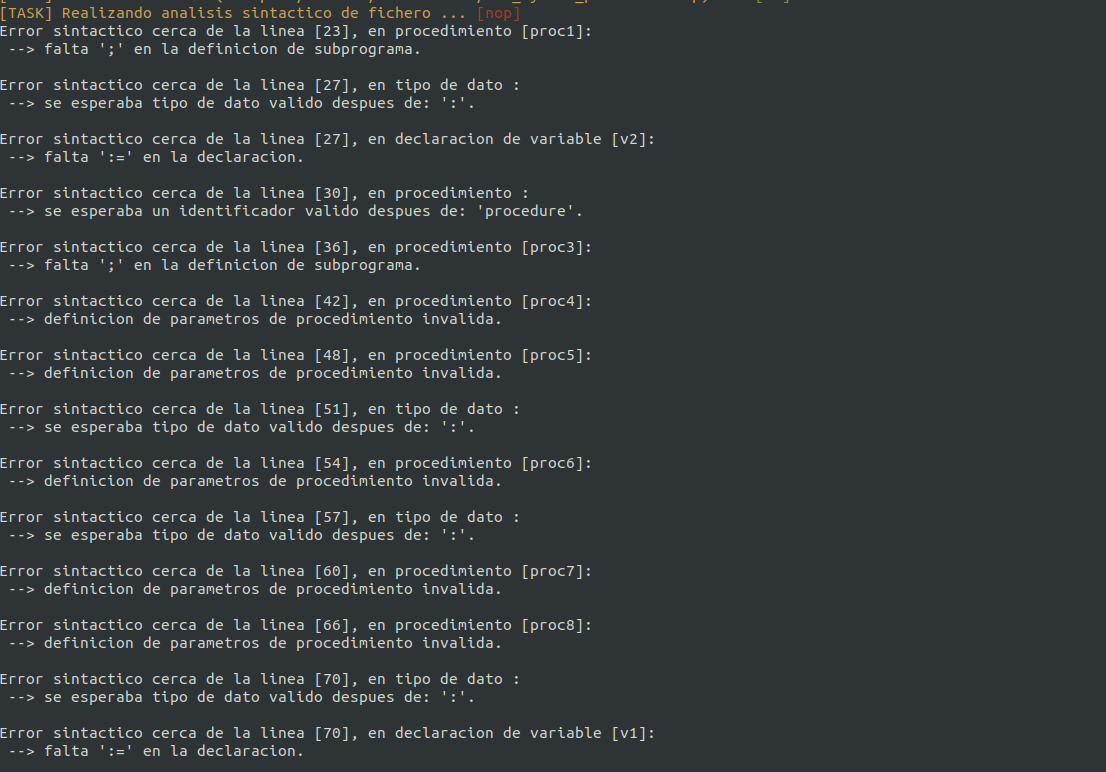
\includegraphics[width=\linewidth]{images/ejemplos/err_syntax/procedures.png}
    \caption{Ejecución de err\_syntax\_procedure.lmp.}
    \label{fig:lamportErrSintaxProcedure_exec}
\end{figure}

\newpage
\subsection{Ejemplo 3: Errores semánticos: uso de variable no definida}
\begin{lstlisting}[style=lamportStyle]
{Fichero: undef_variable.lmp}
{Autor: Daniel Perez Ruiz}
{Descripcion: Contiene un error semantico de tipo: uso de variables no definidas}

program OperaEnteros

function suma(a: integer, b: integer) : integer;
begin
	{ERROR: Uso de variable no definida: resultadoSuma}
	resultadoSuma := a+b;
	return resultadoSuma;
end

procedure resta(a: integer, b: integer);
	var resultado : integer;
begin
	{ERROR: Uso de variable no definida: c}
	resultado := a - c;
	print(resultado);
end

process Main;
begin
	{ERROR: Uso de variable no definida: resultado}
	resultado := suma(3,5);
	{ERROR: Uso de variable no definida: num2}
	resta(3,num2);
end
\end{lstlisting}
\begin{figure}[h]
\caption{Programa Lamport: Errores semánticos (err\_undef\_variable.lmp)}
\label{fig:lamportErrSemanticUndef}
\end{figure}

\newpage
\begin{figure}[h]
    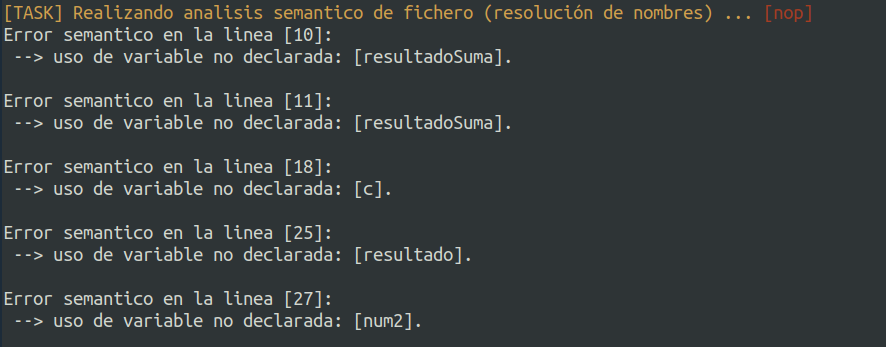
\includegraphics[width=\linewidth]{images/ejemplos/err_semantic/undef.png}
    \caption{Ejecución de err\_undef\_variable.lmp.}
    \label{fig:lamportErrSemanticUndef_exec}
\end{figure}

\newpage
\subsection{Ejemplo 4: Errores semánticos: redefinición de variable}
\begin{lstlisting}[style=lamportStyle]
{Fichero: redef_variable.lmp}
{Autor: Daniel Perez Ruiz}
{Descripcion: Contiene un error semantico de tipo: redefinicion de variable}

program SumaEnteros
	var v1 : integer := 0;
	{ERROR: Redefinicion de variable}
	var v1 : integer;

process Main;
	var resultado : integer := 0;
	{ERROR: Redefinicion de variable}
	var resultado : char;
	{CORRECTO: este v1 esta en otro scope}
	var v1 : string := "hola";
begin
	{Invoca a la funcion para obtener el resultado}
	resultado := v1 + 2;
end
\end{lstlisting}
\begin{figure}[h]
\caption{Programa Lamport: Errores semánticos (err\_redef\_variable.lmp)}
\label{fig:lamportErrSemanticRedef}
\end{figure}

\begin{figure}[h]
    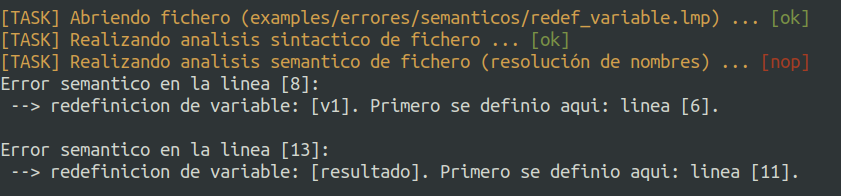
\includegraphics[width=\linewidth]{images/ejemplos/err_semantic/redef.png}
    \caption{Ejecución de err\_redef\_variable.lmp.}
    \label{fig:lamportErrSemanticRedef_exec}
\end{figure}

\newpage
\subsection{Ejemplo 5: Errores semánticos: comprobación de tipos}
\begin{lstlisting}[style=lamportStyle]
{Fichero: typecheck_expressions.lmp}
{Autor: Daniel Perez Ruiz}
{Descripcion: Contiene errores semanticos de typechecking: expresiones}

program Sentencias
	var v1 : boolean := false;
	var v2 : string;
	var v3 : integer;
	
process Main;
	var v4 : real := 8.5;
	var resultado1 : integer;
	var resultado2 : real;
begin
	resultado1 := 1 + 3 * v3 - 1;
	{ERROR}
	resultado2 := v3 + 1.0 - 3;
	{ERROR}
	resultado1 := 1.0 - 10 / 2 + 7.5;
	{ERROR}
	resultado2 := 1 + 5 * 4;
	{ERROR}
	resultado2 := v2 + 3 / 2.5 - 1;
end
\end{lstlisting}
\begin{figure}[h]
\caption{Programa Lamport: Errores semánticos (err\_typecheck\_expr.lmp)}
\label{fig:lamportErrSemanticTypecheck}
\end{figure}

\newpage
\begin{figure}[h]
    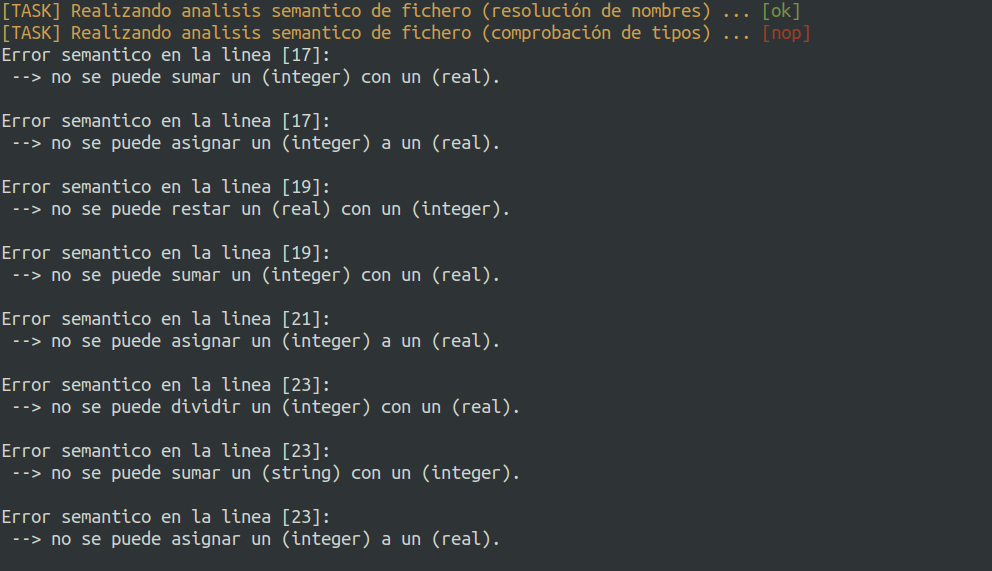
\includegraphics[width=\linewidth]{images/ejemplos/err_semantic/typecheck.png}
    \caption{Ejecución de err\_typecheck\_expr.lmp.}
    \label{fig:lamportErrSemanticTypecheck_exec}
\end{figure}

\newpage
\section{Ejemplos que lanzan excepciones}
Los siguientes ejemplos mostrados son correctos sintácticamente y semánticamente. Sin embargo, realizan operaciones no permitidas, y generan una excepción en el intérprete.

\subsection{Ejemplo 1: Excepción ZeroDivision}
\begin{lstlisting}[style=lamportStyle]
{Programa: zerodivision.lmp}
{Autor: Daniel Perez Ruiz}

program Operaciones
	var num1 : integer := 1;

process Main;
	var num2 : integer := 0;
	var resultado : integer;
begin
	{GENERA EXCEPCION EN LVM: Division zero}
	resultado := num1/num2;
end
\end{lstlisting}
\begin{figure}[h]
\caption{Programa Lamport: Excepción ZeroDivision (zerodivision.lmp)}
\label{fig:lamportExceptionZeroDivision}
\end{figure}

\begin{figure}[h]
    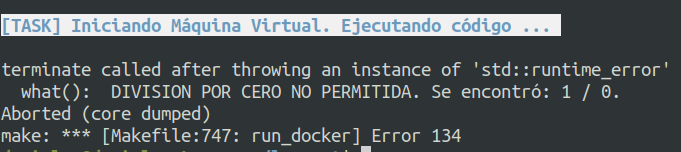
\includegraphics[width=\linewidth]{images/ejemplos/exceptions/zerodivision.png}
    \caption{Ejecución de zerodivision.lmp.}
    \label{fig:lamportExceptionZeroDivision_exec}
\end{figure}

\newpage
\subsection{Ejemplo 2: Excepción IndexOutOfBounds}
\begin{lstlisting}[style=lamportStyle]
{Programa: out_of_bounds.lmp}
{Autor: Daniel Perez Ruiz}

program Arrays
	var numeros : array [5] integer;

procedure negativeBound();
begin
	{EXCEPCION: Se intenta acceder a una posicion negativa de array}
	numeros[-2] := 2;
end

procedure excedBound();
begin
	{EXCEPCION: Se intenta acceder a una posicion negativa de array}
	numeros[6] := -2;
end

procedure printBadArray();
begin
	for i := 0 to 5 do
	begin
		print(numeros[i]);
	end
end
	
{INTERCAMBIE EL ORDEN DE EJECUCION PARA VER LAS EXCEPCIONES}
process main;
begin
	{EXCEPCION TIPO 2: Acceso a region fuera del limite superior}
	excedBound();
	
	{EXCEPCION TIPO 3: Recorrido en bucle que se sale de los limites}
	printBadArray();

	{EXCEPCION TIPO 1: Acceso negativo}
	negativeBound();
end
\end{lstlisting}
\begin{figure}[h]
\caption{Programa Lamport: Excepción IndexOutOfBounds (out\_of\_bounds.lmp)}
\label{fig:lamportExceptionOutOfBounds}
\end{figure}

\newpage
\begin{figure}[h]
    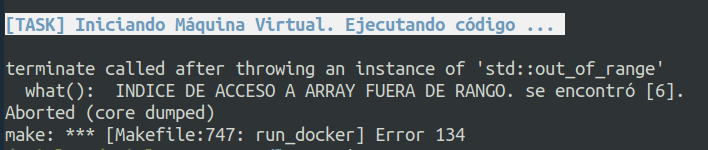
\includegraphics[width=\linewidth]{images/ejemplos/exceptions/out_of_bounds.png}
    \caption{Ejecución de out\_of\_bounds.lmp.}
    \label{fig:lamportExceptionOutOfBounds_exec}
\end{figure}